\documentclass[12pt]{exam}


\usepackage{cmap, type1ec}
\usepackage[T2A]{fontenc}
\usepackage[utf8]{inputenc}
\usepackage[russian]{babel}

\usepackage{xcolor}
\usepackage{hyperref}
\usepackage{alltt}

\hypersetup{%
  colorlinks=false,% hyperlinks will be black
  linkbordercolor=blue,% hyperlink borders will be red
  pdfborderstyle={/S/U/W 1}% border style will be underline of width 1pt
}

\usepackage[margin=1in]{geometry}
\usepackage{amsmath,amssymb}
\usepackage{multicol}
\usepackage{etoolbox}

\usepackage{float}
\usepackage{siunitx}

\usepackage{tikz}
\usetikzlibrary{trees}
\usetikzlibrary{shapes.geometric}
\usetikzlibrary{positioning}

\newcommand{\class}{Теория алгоритмов}
\newcommand{\term}{Весенний семестр 2017}
\newcommand{\examnum}{Пересдача}
\newcommand{\examdate}{2 октября 2017}
\newcommand{\timelimit}{18:10 -- 20:10}

\pagestyle{head}
\firstpageheader{}{}{}
\runningheader{\class}{\examnum\ - Страница \thepage\ из \numpages}{\examdate}
\runningheadrule

\providecommand{\abs}[1]{\left\lvert{#1}\right\rvert}

\renewcommand{\solutiontitle}{}

\makeatletter
\newcommand{\iftoggleverb}[1]{%
  \ifcsdef{etb@tgl@#1}
    {\csname etb@tgl@#1\endcsname\iftrue\iffalse}
    {\etb@noglobal\etb@err@notoggle{#1}\iffalse}%
}
\makeatother

\graphicspath{{./figures/}}

\begin{document}

\noindent
\begin{tabular*}{\textwidth}{l @{\extracolsep{\fill}} r @{\extracolsep{6pt}} l}
\textbf{\class} & \textbf{Студент:} & \makebox[3in]{\hrulefill}\\
\textbf{\term} &&\\
\textbf{\examnum} &&\\
\textbf{\examdate} \\
\textbf{\timelimit}
\end{tabular*}\\
\rule[2ex]{\textwidth}{2pt}%
% \begin{center}
% Оценки (заполняется проверяющими)\\
% \addpoints
% \gradetable[v][questions]
% \end{center}
% \noindent
% \rule[2ex]{\textwidth}{2pt}

\begin{questions}

\question[1] Какое утверждеие верно для очереди, реализованной через связный список?
\begin{checkboxes}
\choice Если {\tt push} добавляет элементы в начало списка, то {\tt pop} удаляет их с конца списка
\choice Если {\tt push} добавляет элементы в конец списка, то {\tt pop} удаляет их из начала списка
\CorrectChoice Всё вышеперечисленное
\choice Ничего из вышеперечисленного
\end{checkboxes}

\question[1] Укажите асимптотическую сложность нахождения 8-го элемента с начала и 8-го элемента с конца в {\em односвязном} списке. Считайте, что в списке $n$ элементов, при этом $n > 8$.
\begin{checkboxes}
\CorrectChoice $O(1)$ и $O(n)$
\choice $O(1)$ и $O(1)$
\choice $O(n)$ и $O(1)$
\choice $O(n)$ и $O(n)$
\end{checkboxes}

\question[1] Что из перечисленного {\em не является} in-place алгоритмом?
\begin{checkboxes}
\choice Insertion sort
\choice Selection sort
\CorrectChoice Merge sort
\choice Heap sort
\end{checkboxes}

\question[1] Пусть даны указатели на первый и последний элементы {\em односвязного} списка. Для какой операции время выполнения будет зависеть от длины списка?
\begin{checkboxes}
\choice Удаление элемента с начала списка
\choice Добавление элемента в начало списка
\CorrectChoice Удаление элемента с конца списка
\choice Добавление элемента в конец списка
\end{checkboxes}

\question[1] Пусть $X$ -- вершина бинарного дерева. $X$ имеет два потомка. Известно, что при in-order обходе за вершиной $X$ сразу последовала вершина $Y$. Что можно сказать про $Y$?
\begin{checkboxes}
\choice $Y$ не имеет правого потомка
\CorrectChoice $Y$ не имеет левого потомка
\choice $Y$ имеет оба потомка
\choice Ничего из вышеперечисленного
\end{checkboxes}

\question[2] Даны три последовательности вершин некоторого бинарного дерева:
$$
\begin{gathered}
(1)~~~MBCAFHPYK\\
(2)~~~KAMCBYPFH\\
(3)~~~MABCKYFPH\\
\end{gathered}
$$
Они соответствуют in-order, post-order, и pre-order обходам одного и того же дерева, но неизвестно соответствие между обходами и последовательностями. Выберите верное утверждение:
\begin{checkboxes}
\choice $(1)$ -- pre-order, $(2)$ -- in-order
\choice $(1)$ -- pre-order, $(3)$ -- post-order
\choice $(2)$ -- in-order, про остальные ничего сказать нельзя
\CorrectChoice $(2)$ -- pre-order, $(3)$ -- in-order
\end{checkboxes}

\question[1] Пусть в бинарном дереве поиска содержатся числа от 1 до 100, и мы хотим найти в нём число 55. Какую последовательность вершин {\em невозможно} получить при таком поиске?
\begin{checkboxes}
\choice {\tt {10, 75, 64, 43, 60, 57, 55}}
\choice {\tt {90, 12, 68, 34, 62, 45, 55}}
\CorrectChoice {\tt {9, 85, 47, 68, 43, 57, 55}}
\choice {\tt {79, 14, 72, 56, 16, 53, 55}}
\end{checkboxes}

\question[1] Дана пустая хэш-таблица размера 10, использующая открытую адресацию со стратегией linear probing. Используется хэш-функция $h(k) = k \mod 10$. После вставки шести элементов хэш-таблица выглядит так:
\begin{figure}[H]
  \begin{center}
    \begin{tabular}{|c|c|c|c|c|c|c|c|c|c|}
    \hline
    0 & 1 & 2  & 3  & 4  & 5  & 6  & 7  & 8 & 9 \\ \hline
    ~ & ~ & 42 & 23 & 34 & 52 & 46 & 33 & ~ & ~ \\ \hline
    \end{tabular}
  \end{center}
\end{figure}
В каком порядке могли быть вставлены эти элементы?

\begin{checkboxes}
\choice {\tt 46, 42, 34, 52, 23, 33}
\choice {\tt 34, 42, 23, 52, 33, 46}
\CorrectChoice {\tt 46, 34, 42, 23, 52, 33}
\choice {\tt 42, 46, 33, 23, 34, 52}
\end{checkboxes}

\question[1] Какое максимальное число рёбер может быть в ациклическом ненаправленном графе с $n$ вершинами?
\begin{checkboxes}
\CorrectChoice $n-1$
\choice $n$
\choice $n+1$
\choice $2n-1$
\end{checkboxes}

\question[1] Какое утверждение верно, если алгоритм $X$ асимптотически более эффективен чем $Y$?
\begin{checkboxes}
\choice $X$ быстрее на всех входных данных
\CorrectChoice $X$ быстрее на всех данных кроме, разве что, данных малого размера
\choice $X$ быстрее на всех данных кроме, разве что, данных крупного размера
\choice $X$ быстрее на на входных данных малого размера
\end{checkboxes}

\question[2] Предположим, что операция перестановки элементов в массиве стала очень дорогой. Какой из алгоритмов сортировки в общем случае выполняет минимальное количество операций перестановки? 
\begin{checkboxes}
\choice Heap Sort
\CorrectChoice Selection Sort
\choice Insertion Sort
\choice Merge Sort
\end{checkboxes}

\question[1] Какой из алгоритмов сортировки работает наименьшее время в случае когда все сортируемые элементы равны?
\begin{checkboxes}
\CorrectChoice Insertion Sort
\choice Heap Sort
\choice Merge Sort
\choice Selection Sort
\end{checkboxes}

\question[2] Что из перечисленного {\em не может} быть последовательностью добавления рёбер при вычисления минимального покрывающего дерева в данном графе с помощью алгоритма Краскала?
\begin{figure}[H]
  \begin{center}
    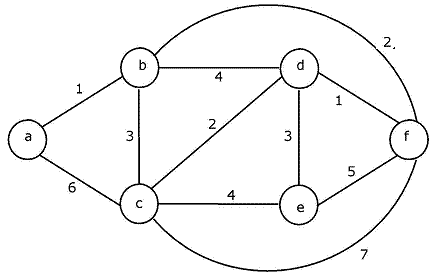
\includegraphics[width=10cm]{mst.png}
  \end{center}
\end{figure}
\begin{checkboxes}
\choice {\tt (a—b),(d—f),(b—f),(d—c),(d—e)}
\choice {\tt (a—b),(d—f),(d—c),(b—f),(d—e)}
\choice {\tt (d—f),(a—b),(d—c),(b—f),(d—e)}
\CorrectChoice {\tt (d—f),(a—b),(b—f),(d—e),(d—c)}
\end{checkboxes}


\question[2] Пусть $G$ -- ненаправленный связный граф, в котором все рёбра имеют различные веса. Пусть $E_{max}$ -- ребро с максимальным, а $E_{min}$ -- минимальным весом. Какое из утверждений {\em неверно}?
\begin{checkboxes}
\choice Каждое минимальное покрывающее дерево (MST) для $G$ обязательно содержит $E_{min}$
\choice Если $E_{max}$ содержится в MST, то при удалении $E_{max}$ $G$ перестанет быть связным
\choice Для $G$ не существует MST содержащих $E_{max}$
\choice Для $G$ существует лишь одно MST
\end{checkboxes}

\question[2] Пусть реализован поиск в ширину, где для хранения соседних вершин используется очередь. Обходим граф:
\begin{figure}[H]
  \begin{center}
    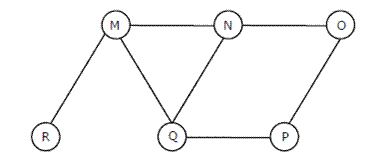
\includegraphics[width=10cm]{bfs.png}
  \end{center}
\end{figure}
Какой из перечисленных путей возможен при таком обходе?
\begin{checkboxes}
\choice MNOPQR
\choice NQMPOR
\CorrectChoice QMNPRO
\choice QMNPOR
\end{checkboxes}

\end{questions}

\end{document}
